\section{A Short Introduction and Motivation}
A pivotal ingredient in the study of strongly correlated systems are real-time correlation functions since they allow us to access the real-time dynamics of the theory at hand. In the context of QCD this includes for example transport phenomena relevant in the study of heavy-ion collisions \cite{AyikNorenbergWolschin1977, Xu2019}.\\  Our theoretical understanding of the non-perturbative sector of QCD has greatly improved during the last decades, mainly due to the complementary efforts and advances in the application of lattice techniques \cite{Philipsen2007, deForcrand2010} and the application of Functional Methods such as the Functional Renormalization Group (FRG) \cite{Wetterich1992, Pawlowski2005} or Dyson-Schwinger equations (DSEs) \cite{Dyson1949, Schwinger1951}. The latter one will be the tool of our choice throughout this work. \\
Despite the advances in the field, the direct computation of these real-time quantities has turned out to pose several problems. We want to tackle this challenging task by making use of the newly developed technique of spectral renormalization \cite{Horak2019, Wink2020, HorakPawlowskiWink2020}, allowing for the direct computation of real-time correlation functions from their respective spectral representations.\\
 The next pages serve as a short introduction to the absolute basics needed for a general understanding of the conducted calculations. The reader familiar with functional methods, the basics of QCD and the K\"allen-Lehmann spectral representation might skip the remainder of this section in a first read. Note, that in general we will not focus on the technical details but rather try to present the most important conceptual steps of the conducted calculations.
\subsection{Functional Methods in Quantum Field Theory}
The central object in functional approaches is the  quantum effective action $\Gamma[\phi]$, directly related to the generating functional $Z[J]$ via a Legendre transform,
\begin{equation}
	\Gamma[\phi]=\sup _{J}\left\{\int_{x} J(x) \phi(x)-W[J]\right\}=\int_{x} J_{\mathrm{sup}}(x) \phi(x)-W\left[J_{\mathrm{sup}}\right],
\label{eqn:Def_Gamma}
\end{equation}
where $W[J] = \ln Z[J]$, the Schwinger functional, the generating functional of the connected correlation functions. $\Gamma[\phi]$ generates the one-particle irreducible (1PI) correlation functions via functional derivatives w.\,r.\,t. the fields, i.\,e.
\begin{align}
	\Gamma^{(n)}[\phi]\left(p_{1}, \ldots, p_{n}\right)=\frac{\delta^{n} \Gamma[\phi]}{\delta \phi\left(p_{1}\right) \cdots \delta \phi\left(p_{n}\right)}.
\end{align}
Here we presented the momentum space expression. The most important quantity for various applications of functional methods is the field-dependent propagator, given by the inverse of the 1PI two-point function,
\begin{equation}
	G[\phi](p,q) = \frac{1}{\Gamma^{(2)}}[\phi](p,q).
\end{equation}
The path integral measure of the generating functional is invariant under field independent spacetime translations $\phi(x) \rightarrow \phi(x) + \Lambda(x)$ and so are the respective correlation functions. The corresponding symmetry identity derived from this is given by
\begin{equation}
\frac{\delta \Gamma[\phi]}{\delta \phi(x)}=\frac{\delta S[\phi]}{\delta \varphi(x)}\left[\varphi=G \cdot \frac{\delta}{\delta \phi}+\phi\right]. \label{eqn:DSE}
\end{equation}
This is the famous Dyson-Schwinger equation (DSE), the central functional relation in the context of our work. More formal derivations can for example be found in  \cite{NPgaugeLecture, AlkoferVonSmekal2000}. Here, $S[\phi]$ is the classical action of the theory at hand, $\phi=\langle\varphi \rangle$ and
\begin{equation}
	G\cdot\frac{\delta}{\delta\phi} = \int\frac{\dd^dq}{(2\pi)^d}\ G(p,q)\frac{\delta}{\delta\phi} .
\end{equation}
This explains how we can extract the correlation functions from the DSE, i.\,e. by taking functional derivatives of equation (\ref{eqn:DSE}). The two-point function is therefore obtained by taking a single field derivative. For the quark propagator in QCD, we depict the corresponding one-loop equation in the typical diagrammatic notation in Figure \ref{fig:dse} at the beginning of the next page. It relates the full (inverse) two-point function to the bare propagator plus higher loop order diagrams, in our case the one-loop quark self energy $\Sigma(p^2)$.
\subsection{Relevant Basics of Quantum Chromodynamics}
Quantum Chromodynamics, the theory of strong interactions, is formulated as a $SU(N_c)$ gauge theory, where $N_c$ refers to the number of colors.
The relevant action functional $S_{\mathrm{QCD}}[\phi]$ for QCD in the Landau gauge reads
\begin{equation}
S_{\mathrm{QCD}}[\phi]=\frac{1}{4} \int_{x}\left\{F_{\mu \nu}^{a} F_{\mu \nu}^{a}+\frac{1}{2 \xi}\left(\partial_{\mu} A_{\mu}^{a}\right)^{2}-\bar{c}^{a} \partial_{\mu} D_{\mu}^{a b} c^{b}+\bar{q}\left(i\slashed{D}+m_{q}\right) q\right\},
\label{eqn:S_QCD}
\end{equation}
with the usual conventions for the non-Abelian field strength $F_{\mu\nu} = F_{\mu\nu}^{a}T^{a}$ with the generators of the gauge group  $T^{a} \in SU(N_c)$ and 
\begin{equation}
	F_{\mu \nu}^{a}=\partial_{\mu} A_{\nu}^{a}-\partial_{\nu} A_{\mu}^{a}+g f^{a b c} A_{\mu}^{b} A_{\nu}^{c}.
\end{equation}
Here $f^{abc}$ are the structure constants, $g$ is the strong coupling constant and  $A_{\mu}^{a}$ is the gluon field. The other terms are the usual gauge fixing term with gauge fixing parameter $\xi$,the ghost term with the ghost and anti-ghost fields $c^{a}$ and $\bar{c}^{a}$ and the Dirac or matter part consisting of the fermionic quark and anti-quark fields $q$ and $\bar{q}$ and the respective covariant derivatives and mass terms. A summary of the Feynman rules following from the given action can be for example found on the appendix of \cite{NPgaugeLecture}.
Landau gauge is achieved by the choice $\xi\rightarrow 0$. This gauge choice is particularly useful since it   allows for a decoupling and closure of the system of all the transverse correlation functions. The pure gauge, or Yang-Mills sector of QCD is currently studied in our group using the same methods as presented here, first results have been published just recently \cite{HorakPapavassiliouPawlowskiWink2021}.
\begin{figure}[t]
\centering	
\begin{align*}
\bigg(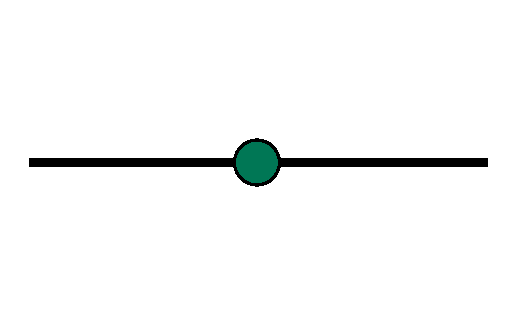
\includegraphics[scale=0.4, valign=c]{figures/full_quark_propagator}\bigg)^{-1} = 
\bigg(
\includegraphics[scale=0.4, valign=c]{figures/bare_quark_propagator.pdf}\bigg)^{-1} - 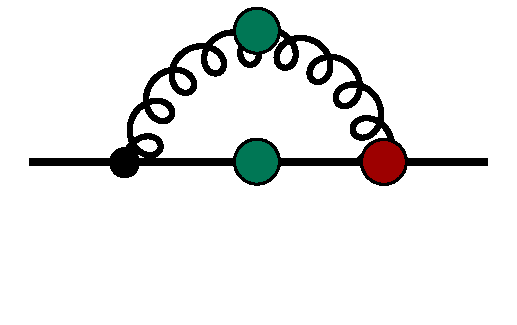
\includegraphics[scale=0.4, valign=c]{figures/quark_self_energy}
\end{align*}
\caption{Diagrammatic representation of the quark propagator DSE. Green blobs indicate full propagators, red blobs full vertices and black dots the respective classical counterparts.}
\label{fig:dse}
\end{figure}

\subsection{K\"allen-Lehmann Spectral Representation}
The K\"allen-Lehmann spectral representation \cite{Kallen1952, Lehmann1954} allows us the recast the propagator, or more general arbitrary correlation functions, in terms of a spectral integral over the respective spectral function $\rho(\lambda)$ with spectral parameter $\lambda$\footnote{Note that we choose to work with the convention of a spectral function of a linear argument $\lambda$ instead of $\lambda^2$ which is often found in the literature. This is achieved simply by changing the integration variable from $\dd\lambda^2 \rightarrow \lambda\ \dd\lambda$.} as follows:
\begin{align} 
G(p)=\int_{0}^{\infty} \frac{\dd \lambda}{\pi} \frac{\lambda\rho(\lambda)}{p^{2}+\lambda^{2}}. \label{eqn:KL_rep}
\end{align}
This can be interpreted as an integral over classical free propagators of a particle with squared mass $\lambda^2$ weighted by the spectral density $\rho(\lambda)$, or for the case of asymptotic states, as probability density for the transition to an excited state with energy $\lambda$. The spectral density $\rho(\lambda)$ encodes all the information about the energy spectrum of the theory. An example spectral function in the context of a scalar theory is visualized in Figure \ref{fig:scalar_spec_func}.\\
In terms of a mathematical interpretation, the spectral function arises as the set of non-analycities of the propagator, whose locations in the complex plane are restricted by Cauchy's theorem. From this an inverse relation between the retarded propagator and the spectral function can be derived. It reads
\begin{equation}
	\rho(\omega, \abs{\vec{p}}) = 2 \operatorname{Im}\left[G\left(-i(\omega + i0^+), \abs{\vec{p}}\right)\right], \label{eqn:specfunc_relation}
\end{equation}
with $\omega$ being the zero component of the real-time momentum. Note, that due to the requirement of Lorentz invariance we do not need to consider the spatial momentum explicitly since all kinetic information can be restored from Lorentz invariance. Hence will we drop it for the remainder of this work. This relation is of particular importance, since we will use it later on to extract the spectral function from the computed retarded propagator. \\ 
\begin{figure}[t]
\centering
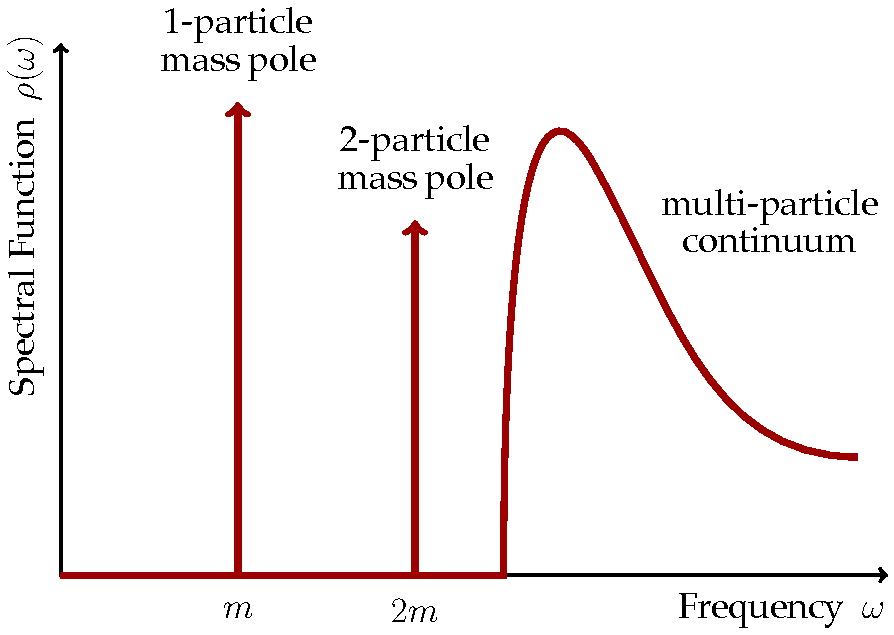
\includegraphics[width=0.6\textwidth]{figures/scalar_spec_func}
\caption{Shape of a typical spectral function of a scalar theory. The isolated poles of the propagator show up as delta peaks in the spectral function. The continuous tail is generated by branch cuts. The visualization is inspired by \cite{NPgaugeLecture}.}\label{fig:scalar_spec_func}
\end{figure}

\noindent 
From equations (\ref{eqn:KL_rep}) and (\ref{eqn:specfunc_relation}) it follows straightforwardly, that all the non-analycities of the propagator are restricted to the real momentum axis. This allows us to split the spectral function into pole contributions and a continuous (scattering) part generated by branch cuts, i.\,e.
\begin{equation}
	\rho(\lambda) = \frac{\pi}{\lambda}\sum\limits_{i} Z_i\ \delta(\lambda-m_i) + \rho_{\mathrm{cont}}(\lambda). \label{eqn:split}
\end{equation}
From this ansatz the spectral function reproducing the classical propagator is simply obtained from equation (\ref{eqn:split}) by setting $Z_1 = 1$, $Z_{i>1} = 0 $ and $\rho_{\mathrm{cont}}=0$.\\
With this relatively simple structure at hand we can now move on to the explicit details of the conducted computations. The next section is denoted to the introduction of the important features of the spectral renormalization scheme.







